\subsection{Kubernetes} \label{kubernetes}
Kubernetes is the de-facto standard for container orchestration and the main aspect of this thesis. In this section I look at the fundamentals of Kubernetes and highlight the best strategies to run it on edge devices. I will also look what is currently missing to make it a truly edge ready. With that being said, Kubernetes has so many features and tools that discussing them all is impossible. The same is true for its ecosystem which is constantly evolving and adding even more layers to the mix. I will try to keep this section short and concise, but it will come at the cost of complexity.\\
IIoT has accelerated the need for fog computing and the industry is set to develop a container based orchestration tool, tightly integrated with Kubernetes. The Kubernetes IoT edge working group was set up specifically to find the optimal Kubernetes strategy for the edge. However, it is not clear, whether the solution will be Kubernetes itslef or a more specialized tool. In this thesis I will argue that Kubernetes is the way forward as it already posses many of the features that are need for the edge.\\ 
I will start by addressing the elephant in the room, single-cluster vs multi-cluster. I will then analyze the core components of Kubernetes, mainly the kubelet, together with other resource configurations. Finally, I will focus on the optimal deployment strategy, how to control and secure resources on the edge and how to select nodes.

\subsubsection{Single Vs Multi-Cluster}
Google recently revealed a new and much hyped product, Anthos\cite{TechnicalAnthosGoogle66:online}. Its a combination of many services, but most importantly it lets people easily manage hybrid clouds. Google describes it as follow: "Anthos is a modern application management platform that provides a consistent development and operations experience for cloud and on-prem environments"\cite{TechnicalAnthosGoogle66:online}. Google provides an installer for on-prem but onece installed Google itself manages the cluster including updates and troubleshooting. Not only is it a multi-cluster solution, but it also integrates the clusters with Istio service mesh and other neat features. Open source Kubernetes only has the multi-cluster management solution called Kubernetes Cluster Federation.



\subsubsection{Core Components}
Kubernetes is complex to say the least. However, much of the complexity stems from the control plane which only runs on the master nodes. These nodes are not in the scope of this thesis and thus not explained in more detail. Worker nodes on the other hand are orchestrated and provide their state to the master. This is a lot less resource intensive and there are a few tricks to reduce the resource load even further. But first, for a node to be part of a cluster it needs to run the following components: the \textit{kubelet}, \textit{kube-proxy} and a supported container runtime. How Kubernetes works in practice can be seen in \cref{fig:nodeComponents}\footnote{The \textit{cAdvisor} component is a health checking tool and not required.}.
\begin{figure}[h!]
    \centering
    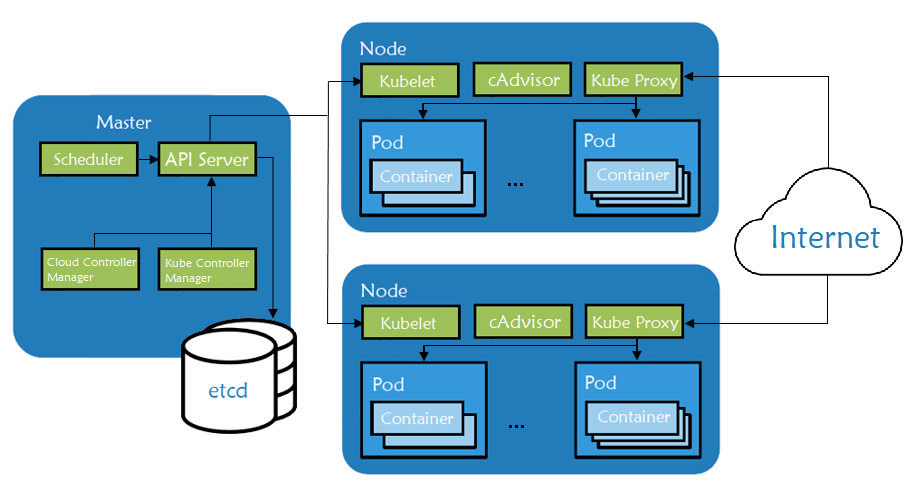
\includegraphics[scale=0.6]{figures/rancherK8sComponents.png}
    \caption{The Kubernetes architecture and node components\cite{nodeSetupKubernetes:online}}
    \label{fig:nodeComponents}
\end{figure}
The kubelet is the primary node agent and schedules and maintains containers running inside a pod based on the pods \textit{PodSpecs}. It gets the these specifications mainly from the APIServer, but other Kubernetes internal sources are possible, too. Containers created outside of Kubernetes are not managed by kubelet. Configuring the kubelet is easily possible via the kubectl and kubeadm tools which give the possibility of enhancing the kubelets performance for different circumstances, here the edge. Going through the possible configurations under \url{https://kubernetes.io/docs/reference/command-line-tools-reference/kubelet/}, the most important configurations for this thesis is the \textit{--housekeeping-interval duration} which defaults to 10s\cite{rancherKubernetesComponents:online}. This means each 10 seconds kubelet performance a complete health check of all its components and sends it to the master. For normal nodes in the cloud, this is fine, but for light edge devices this seems overkill. The k3s kubelet is compatible with Kubernetes and optimized for light edge devices.\\
The kube-proxy is a network proxy node agent ensuring that the Kubernetes networking services runs on each node. It enables the Kubernetes service abstraction by ensuring the network rules on the host and carries out the connection forwarding. The last component, the container runtime, ensures that containers can run as expected. Both components are not from major importance in this thesis.




\subsubsection{Deployment Strategies}
\comment{
deployment vs statefulset vs daemonset
Taints, nodeselector, affinities
namespaces
}
https://kubernetes.io/blog/2018/01/core-workloads-api-ga/

\comment{
Removed section: Security and Recommendations
}